\section{Teststation software}
\label{sec:sw}

The software implemented to run the teststation essentially consists of two programs running in parallel: one taking care of the DAQ and immediate data analysis, one devoted to the slow control of the climatic chamber. 

\subsection{DAQ, Run control and test scenarios}

The ARC boards are operated with a software which is based on ARCS version 6.1~\ref{sec:arcs} and~\ref{sec:acdc}.\\
The modified ARCS version fulfills the special needs for the test station: in particular the teststation ARCS is able to perform the test on all the loaded hybrids, implements the pulse injection test and 
has been modified to interact with the slow control application in such a way tests are performed automatically once the desired environmental condition have been reached. The entire test procedure can proceed without the intervention of the operator that is only asked to load and unload the hybrids. The test scenario is given to ARCS trough a simple text file in which the sequence of operations is coded with a specific format
Beyond the high automatization, to facilitate the operator also a simple and intuitive interface has been implemented where the operator only needs to scan the bar codes of the hybrids. A screenshot of the software is shown in figure~\ref{fig:ss_arcs_teststation}.
\begin{figure}[h]
  \begin{center}
    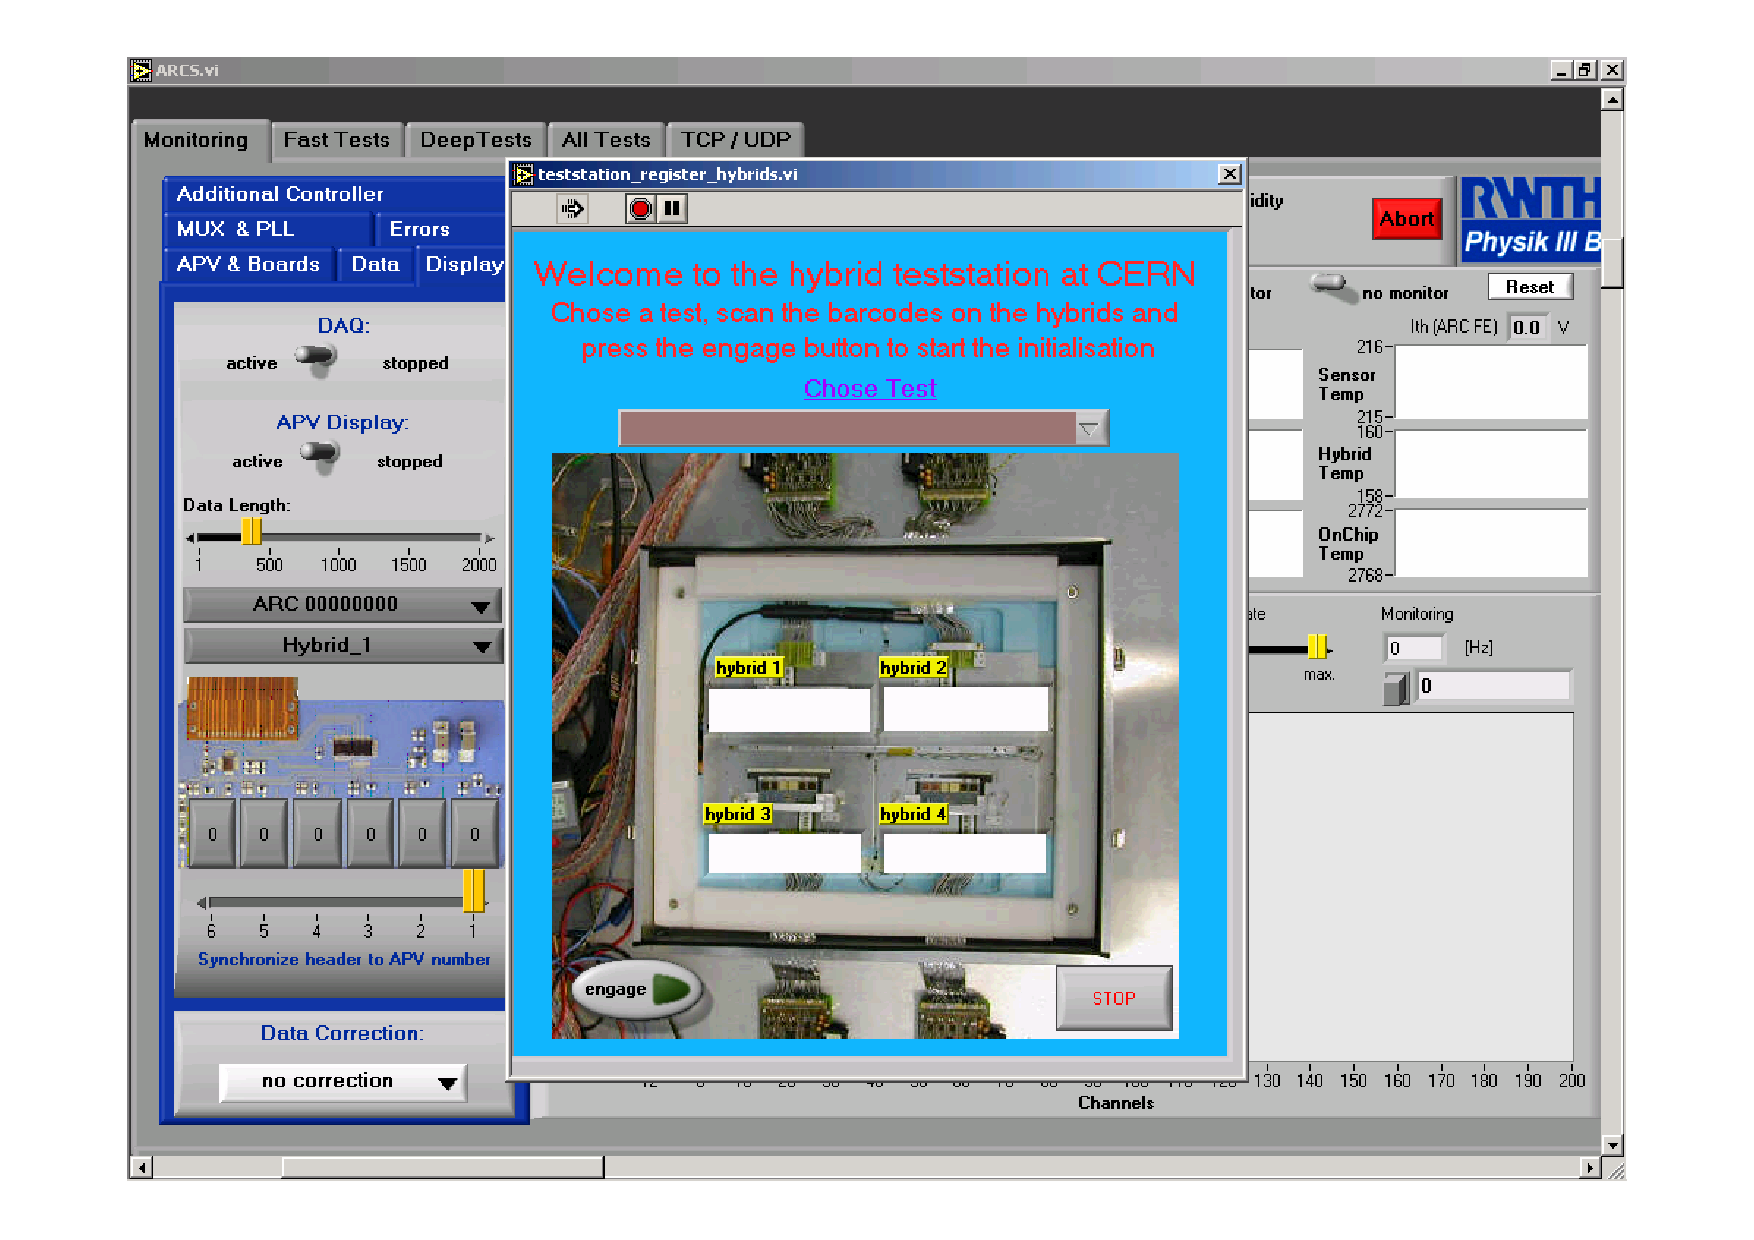
\includegraphics[width=\textwidth]{fig/ss_arcs_hybrid_test_station_mod.pdf}
%\includegraphics*[width=0.99\textwidth]{fig/cms_note.pdf}
    \caption{Screenshot of the ARCS version for the hybrid test station showing the initialization panel were only the bar codes of the hybrids have to be scanned.}
    \label{fig:ss_arcs_teststation}
  \end{center}
\end{figure}

The tests which are performed in the hybrid test station are a pedestal and noise test, a calibration pulse test at fixed timing position and the pitch adapter signal injection test.

At the end of a test, the DAQ software immediately gives to the operator feedback on the hybrid test result on the basis of the quality criteria described in~\ref{sec:}. The test results are automatically uploaded to the Tracker Construcrion Database.

\subsection{Slow control}
\label{sec:slowcontrol}
\label{sec:acdc}

The main application for controlling the environmental conditions inside the hybrid test station is called ACDC. 
The software monitors and controls the temperature and the humidity of the test box and provides flags that can be queried by the ARCS system.
In this way the tests can be started when the desired temperatures are reached.
ACDC also gives alerts if any parameter leaves the range of safe operation. 
The temperature control is done regulating the current and the polarity of the peltier element. 
The difference between the actual temperature readings with respect to the required temperature are fed into a software implemented PID filter that returns the current value, signed (i.e. cooling or heating), that has to be driven into the peltier element through the cooli box and its built-in polarity switch.
\begin{figure}[h]
  \begin{center}
    \resizebox{\textwidth}{!}{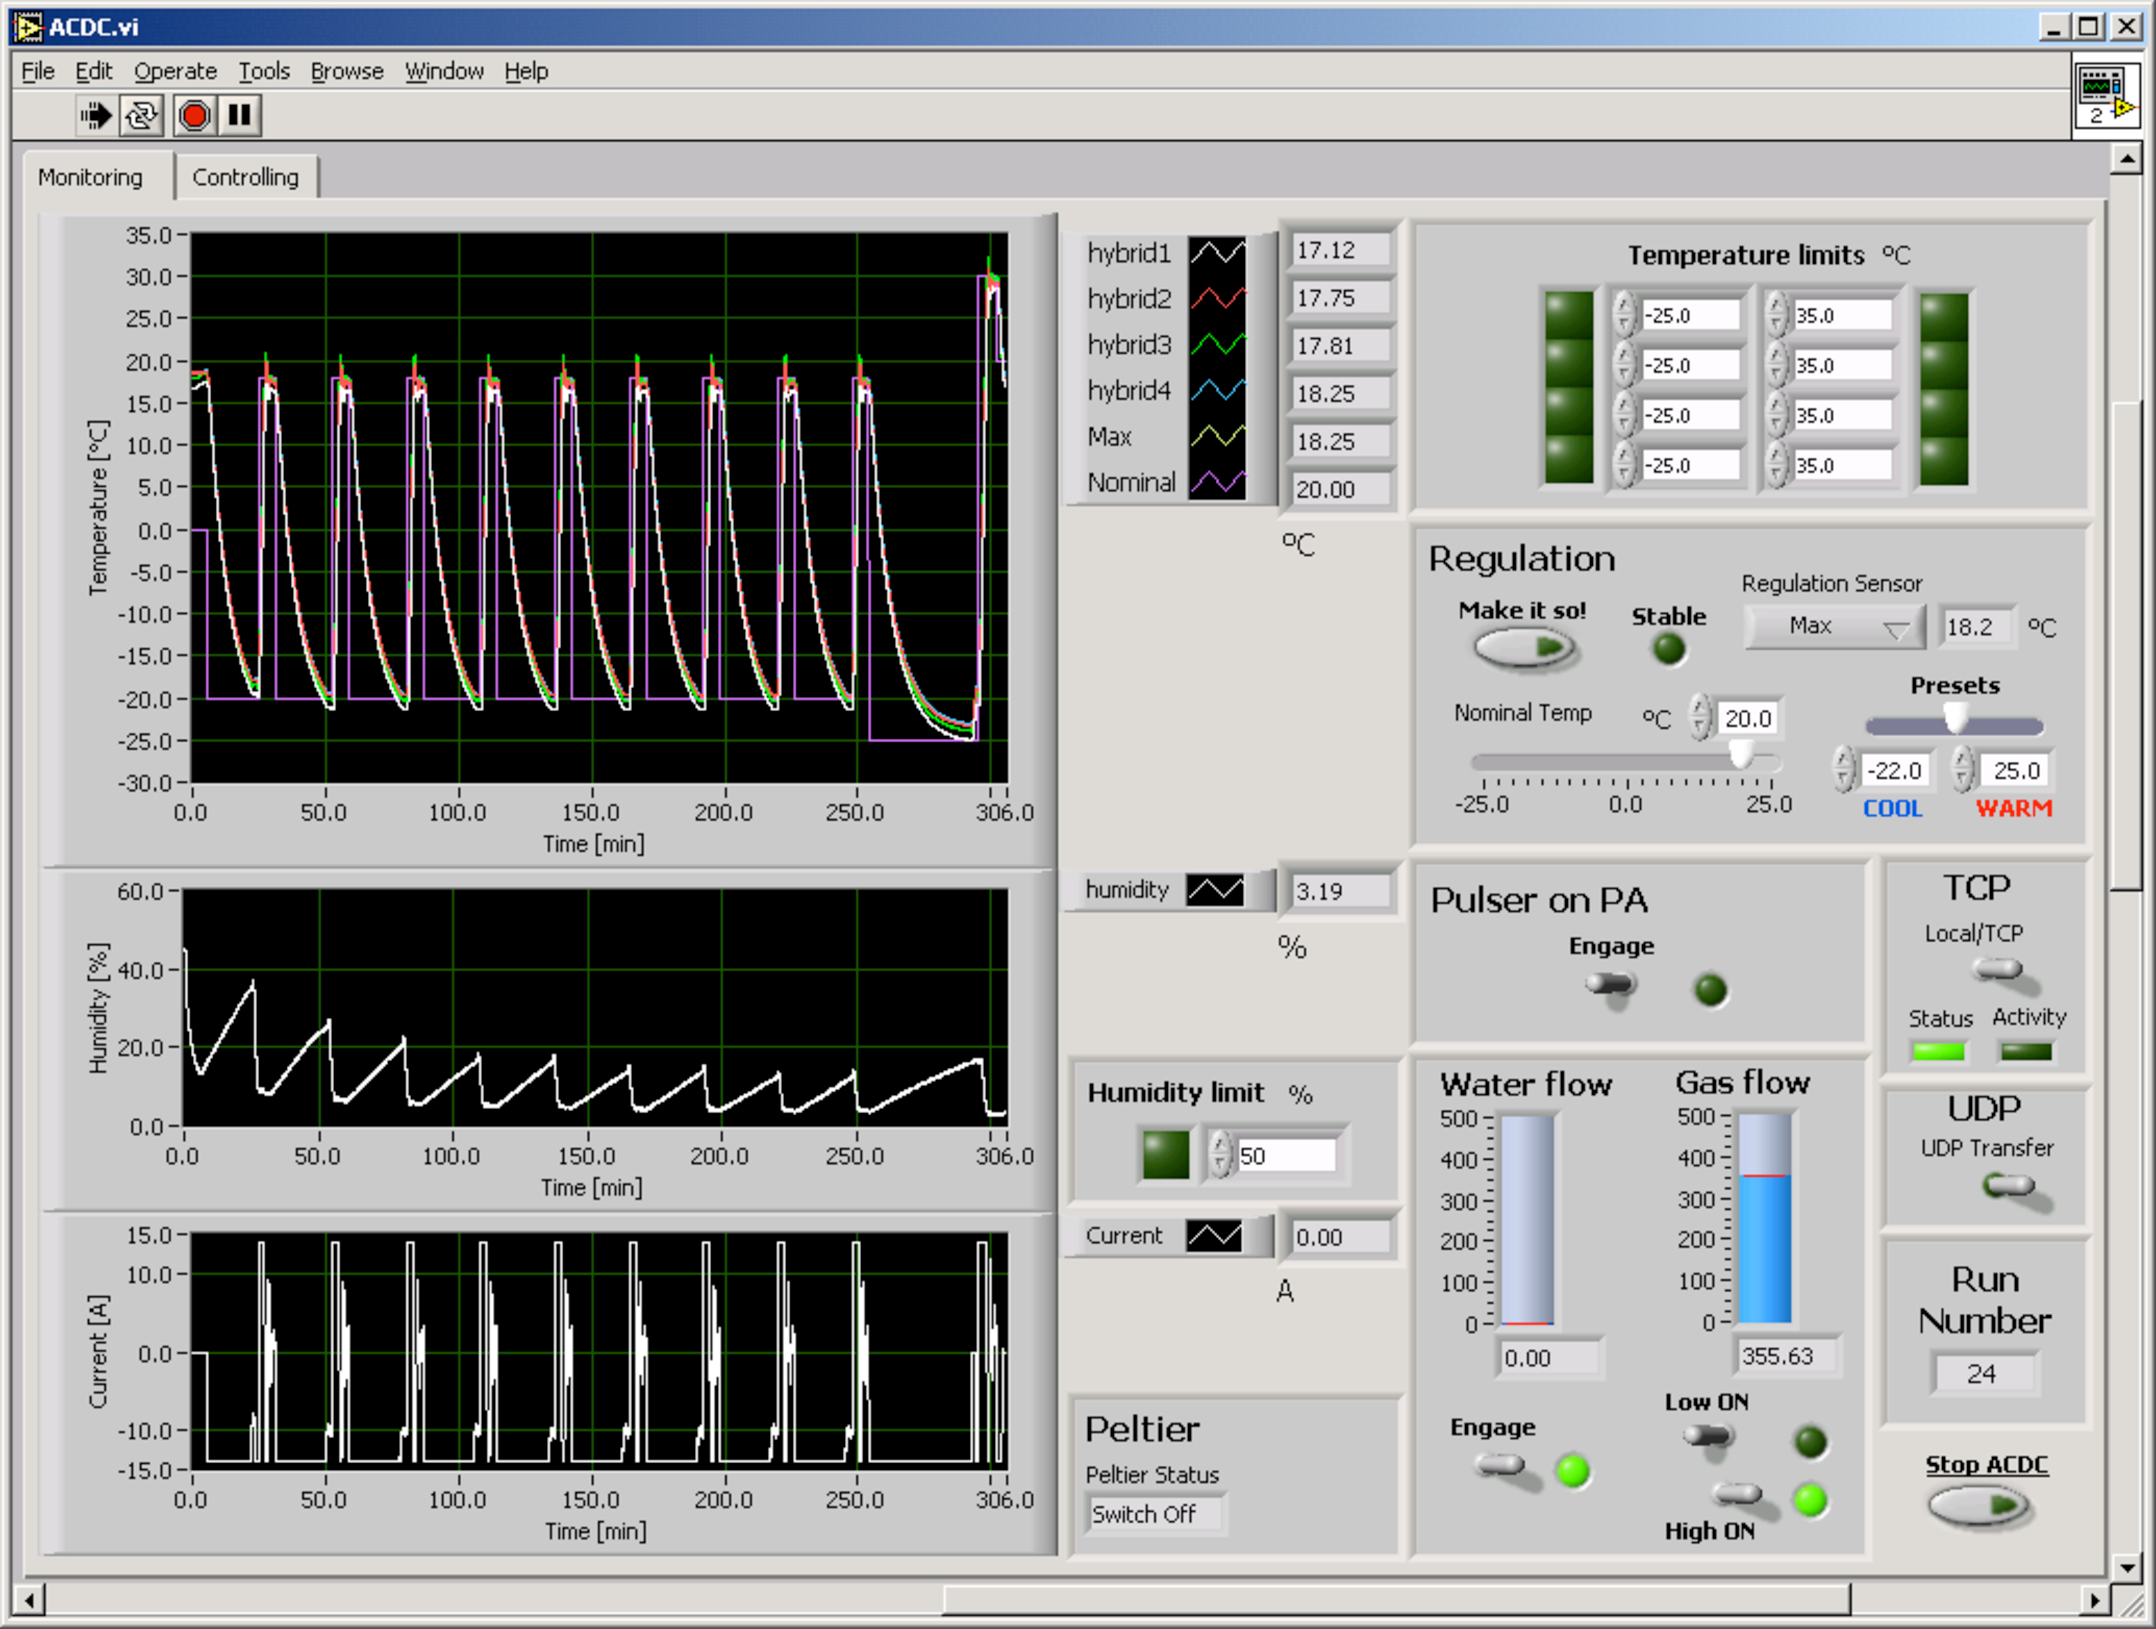
\includegraphics{fig/ACDC_screenshot.pdf}}
    \caption{Screenshot of the ACDC version for the hybrid test station.}
    \label{fig:ss_acdc_teststation}
  \end{center}
\end{figure}
ACDC cycles trough all the temperature sensors every second and the {\em Partial-Integral-Differential}, {PID}, filter is implemented as follows: 
\begin{equation}
J_\mathrm{Peltier} = P\cdot\left( T - T_{\rm set}\right) + I \cdot \left( T - T' \right) \left( t-t' \right) + D\cdot \frac{T - T '}{t-t'},
\label{eq:pid}
\end{equation}
where:\\
- $T_{\rm set}$, target temperature;\\
- $T$, last temperature reading;\\
- $T'$, preavious temperature reading;\\
- $t$, time of last reading;\\
- $t'$, time of preavious reading;\\
- $J_\mathrm{Peltier}$, current made flowing into the Peltier element; the sign convention is such that negative current means 'cooling';\\
- $P$, $I$ and $D$, coefficients of the proportional, integral and differential components of the filter, respectively.

The {\em temperature reading} is the temperature choosen as the {\em regulated temperature}, i.e. the temperature to be set at the {\em target temperature}. Since the test-station features one temperature sensor per hybrid slot, the default regulated temperature is just the maximum temperature reading among the four hybrid sensors. For special runs (i.e. without all the four hybrids), ACDC allowed any of the temperatures of the sensors sitting into the test-station to be choosen as regulated temperature.

The values of the filter component coefficients have been choosen to minimize the time to reach the target temperature while keeping under control over/undershoots and oscillations around the $T_{\rm set}$ value. Two different sets of coefficients have been used depending on the $T_{\rm set}$ ranges used for the tests ($T_{\rm set}>10\Cdegree$ and $T_{\rm set}<-10\Cdegree$), as a consequence of the very different performance of the test-station set up in heating and cooling. The coefficient values are given in table~\ref{tab:pidcoeff}. Obviously the test-station set up performances in heating are much better than in cooling. This is reflected in the smaller proportional coefficient and in the bigger differential coefficient in case of $T_{\rm set}>10\Cdegree$ with respect to the $T_{\rm set}<-10\Cdegree$ case.
Regardless the output of the PID filter, the current is limited within $\pm 14\A$ according to the specifications of the Peltier element.

\begin{table}[h]
  \centering
  \begin{tabular}{r|c|c|c}
                       & $P$ & $I$ & $D$ \\
    $T_{\rm set}$ range & [$\!\A\Cdegree$] & [$\!\A/(\Cdegree\s)$] & [$\!\A\s/\Cdegree$] \\ \hline
    $T_{\rm set}<-10\Cdegree$ & 14.0 & 0.03 & 0.\\
    $T_{\rm set}>10\Cdegree$ & 8.0 & 0.03 & 18.0\\
  \end{tabular}
  \caption{Values of the coefficients of the PID filter for the temperature ranges of interest for the test station.}
  \label{tab:pidcoeff}
\end{table}

An example of a typical temperature cycle is shown in Fig.~\ref{fig:Tcycle}. To cool down from room temperature to $-20\Cdegree$ about $20\mn$ are needed. Heating up back to $18\Cdegree$ is much faster, needing only about $5 \mn$.

\begin{figure}[h]
  \begin{center}
\includegraphics*[width=0.65\textwidth]{fig/cycle.png}
   \begin{picture}(0,0)
     \put(-255,85){\mbox{(c)}}
     \put(-255,190){\mbox{(b)}}
     \put(-255,395){\mbox{(a)}}
     \put(-258,318){\mbox{\textcolor{blue}{\sf T$_{\sf set}$}}}
     \put(-255,360){\mbox{{\sf T}}}
   \end{picture}
    \caption{Test-station temperature cycle: (a) regulated temperature $T$ and target temperature $T_{\rm set}$; (b) humidity in the climatic chamber; (c) current in the Peltier element.}
    \label{fig:Tcycle}
  \end{center}
\end{figure}

A criterion has been implemented into ACDC to declare the target temperature reached and stable. According to this criterion ACDC issues the 'stable' flag to ARCS in order to start all the tests foreseen at that temperature or to take any other action. The target temperature is declared reached and stable if
\begin{equation}
\sqrt{\left(T-T_{\rm set} \right)^2 + \left( \tau\cdot\frac{T-T'}{t-t'}\right)^2} < 1\Cdegree,
\end{equation}
with the same notation used in eq.~(\ref{eq:pid}). The term proportional to the derivative allows the stability to be estimated within the time span $\tau$. Within the test-station setup a value of $10\s$ has been chosen for $\tau$.  

